\documentclass{article}

% Submission version (double-blind, anonymous)
\usepackage{neurips_2026}

\usepackage[utf8]{inputenc}
\usepackage[T1]{fontenc}
\usepackage{hyperref}
\usepackage{url}
\usepackage{booktabs}
\usepackage{amsfonts}
\usepackage{amsmath}
\usepackage{amssymb}
\usepackage{nicefrac}
\usepackage{microtype}
\usepackage{xcolor}
\usepackage{graphicx}
\usepackage{multirow}
\usepackage{array}
\usepackage{pgfplots}
\pgfplotsset{compat=1.18}

% ----------------------------------------------------------------
% Custom macros
% ----------------------------------------------------------------
\newcommand{\CDI}{\textsc{cdi}}
\newcommand{\CQI}{\textsc{cqi}}
\newcommand{\PhAQ}{\textsc{phaq}}
\newcommand{\ATC}{\textsc{atc\_cqi}}
\newcommand{\CY}{\textsc{cy}}
\newcommand{\CPP}{\textsc{cpp}}
\newcommand{\CIDI}{\textsc{cidi}}
\newcommand{\PISA}{PISA}
\newcommand{\AEC}{\textsc{aec}}
\newcommand{\EN}{\textsc{en}}
\newcommand{\CS}{\textsc{cs}}

% ----------------------------------------------------------------
\title{Epistemic Role Framing Elicits Deep Collaboration in LLM Multi-Agent Systems}

% Anonymous submission — author block omitted
\author{Anonymous Authors}

\begin{document}

\maketitle

% ================================================================
\begin{abstract}
Evaluating whether LLM agents genuinely collaborate---rather than merely
exchange outputs---demands metrics that go beyond task accuracy to
characterise \emph{how} agents reason together. We address this
measurement gap with two contributions: the \textbf{Collaborative Phase
Profile (\CPP)} evaluation framework, grounded in the PISA 2015
Collaborative Problem Solving (CPS) model, which characterises each
dialogue via four metrics (\CDI, \CQI, \PhAQ, \CY); and the
\textbf{Collaborative Interdependence-Directed Information (\CIDI)}
benchmark---a corpus of $140$ MATH problems, each equipped with
\CIDI-generated information packets designed to induce epistemic
interdependence, verified by \AEC{} to achieve both-solo-zero in
$85\%$ of problems, enabling controlled evaluation of collaborative
necessity in an information-split regime.
Using this infrastructure, we investigate \emph{epistemic role framing}:
does instructing agents to adopt the communicative stance of active
learners---rather than expert solvers---shift behavior from
answer-generation toward collaborative sense-making? We compare three
conditions across $1{,}967$ conversations: \textbf{C2} (natural),
\textbf{C6} (peer-aware), and \textbf{C7} (student role).
Student-role framing drives a decisive shift: mean \CDI{} rises from
$0.362$ to $0.613$ ($\Delta = +0.251$, $d = 1.30$, $p \approx 0$) and
fully-coupled collaboration (COUPLING) more than doubles ($11\% \to
24\%$). Peer-awareness alone (C6) yields no practically meaningful
improvement ($d = 0.16$, not significant after Bonferroni correction),
establishing that framing content beyond partner-awareness is necessary
to produce measurable collaborative depth in this regime. C7 numerically
outperforms C2 across all 30 subject $\times$ difficulty cells, though
per-cell sample sizes are small and this is descriptive evidence rather
than formal cell-level generalization.
A Shapley-value decomposition (\textbf{Agent Epistemic Contribution},
\AEC) further distinguishes \emph{structural} interdependence---encoded
by the \CIDI{} split ($85\%$ both-solo-zero)---from \emph{activated}
epistemic necessity, achieved in $25\%$ of problems under the optimal
framing (pair correctness $3.6\times$ solo maximum). This structural vs.\
activated distinction provides a principled vocabulary for diagnosing
benchmark difficulty and framing effects. We release the \CPP{} rubric, \CIDI{} pipeline, conversation logs,
\AEC{} scripts, and a benchmark card documenting corpus conditionality
and intended use, to support reproducibility and future evaluation work.
\end{abstract}

% ================================================================
\section{Introduction}
\label{sec:intro}

Multi-agent systems built on LLMs have demonstrated remarkable
capabilities in code generation \citep{hong2023metagpt}, scientific
reasoning \citep{lu2023mathvista}, and debate-based
refinement \citep{liang2023encouraging}. In most of these systems,
collaboration is designed at the \emph{task level}: agents receive
different tools, different roles in a pipeline, or access to different
data shards. Relatively little attention has been paid to whether the
\emph{epistemic stance} an agent adopts---how it positions itself
cognitively with respect to its own knowledge and its partner's
knowledge---can alter the quality of emergent collaboration.

This question has both evaluation and design implications. On the
evaluation side, benchmarking collaborative agents requires metrics
that can distinguish genuine joint reasoning from efficient
answer-delegation---a distinction that task-accuracy scores collapse.
On the design side, research in the learning sciences has long
established that productive collaboration requires participants to
engage in genuine co-construction of understanding rather than
answer-sharing or expertise-transfer
\citep{roschelle1995construction, dillenbourg1999collaborative}.
If LLM agents default to the role of a knowledgeable assistant---which
is precisely what instruction fine-tuning optimises for---eliciting
collaborative behaviour requires an explicit epistemic intervention,
not merely a task decomposition. Developing and validating such
interventions demands evaluation infrastructure that does not yet
exist for LLM multi-agent systems.

We operationalise this intervention through three increasingly
specific framing conditions (see Section~\ref{sec:design}). The
weakest framing (\textbf{C2}) provides no special instructions beyond
handing each agent a partial information packet. The intermediate
framing (\textbf{C6}) additionally makes agents \emph{aware} that a
peer with complementary information exists. The strongest framing (\textbf{C7}) instructs agents to adopt the
communicative stance of an active student: express uncertainty
explicitly, ask clarifying questions, verify understanding aloud before
advancing to solution steps, and treat the partner's contributions as
material to reason about.

To quantify how deeply agents collaborate, we introduce the
\textbf{Collaborative Phase Profile (\CPP)} framework
(Section~\ref{sec:framework}), grounded in the PISA 2015 CPS
competency model \citep{pisa2015cps}. \CPP{} decomposes each
conversation into a $4 \times 3$ matrix of collaborative phases and
competencies and derives four summary statistics: \CDI{} (breadth of
phase engagement), \CQI{} (quality-weighted depth), \PhAQ{} (quality
of joint exploration), and \CY{} (composite yield).

\paragraph{Contributions.} This paper makes four contributions to the
evaluation and design of LLM multi-agent systems:
\begin{enumerate}
    \item \textbf{The \CPP{} evaluation framework}: a principled,
    reproducible scoring rubric for measuring collaborative depth in
    LLM multi-agent dialogues, grounded in the PISA 2015 CPS competency
    model. \CPP{} provides four complementary metrics (\CDI, \CQI,
    \PhAQ, \CY) and a quadrant taxonomy (COUPLING / PROD\_FAIL /
    TRIVIAL / COLLAPSE) that jointly characterise both process quality
    and outcome.
    \item \textbf{The \CIDI{} benchmark}: an interdependence-controlled
    corpus of $140$ MATH problems with \CIDI-generated packets designed
    to make collaboration structurally necessary, verified by \AEC{}
    to yield both-solo-zero in $85\%$ of problems. The corpus enables
    controlled comparison of framing conditions on problems where
    information-split interdependence is empirically confirmed.
    \item \textbf{Controlled evidence for epistemic role framing}: a
    large-scale ($n = 1{,}967$ conversations) three-condition study
    showing that instructing agents to adopt an active-learner stance
    shifts behavior from expert-answering to collaborative sense-making
    ($d = 1.30$, $p \approx 0$), while peer-awareness alone does not
    ($d = 0.16$, not significant after Bonferroni correction).
    \item \textbf{Structural vs.\ activated interdependence via \AEC}:
    a Shapley-value decomposition that distinguishes whether
    interdependence is merely present in the task design (structural:
    $85\%$ both-solo-zero) versus actually exploited under the optimal
    framing (activated under C7: $25\%$ epistemic necessity rate;
    collaborative surplus $+0.207$)---a diagnostic applicable to any
    multi-agent benchmark using information splitting.
\end{enumerate}

% ================================================================
\section{Background}
\label{sec:background}

\subsection{PISA 2015 Collaborative Problem Solving Framework}

The OECD's PISA 2015 assessment introduced a widely cited framework
that characterises collaborative problem solving along two axes: the
\emph{problem-solving process} (Exploring \& Understanding~[A],
Representing \& Formulating~[B], Planning \& Executing~[C], and
Monitoring \& Reflecting~[D]) and the \emph{collaboration competency}
(Establishing \& Maintaining Shared Understanding~[1], Taking
Appropriate Action to Solve~[2], and Establishing \& Maintaining Team
Organisation~[3]) \citep{pisa2015cps}. Their cross-product defines 12
cells---e.g., \textit{A1}: jointly building an initial problem model,
\textit{D3}: collectively revising the team's shared strategy. PISA
operationalised these cells for human dyads; we adapt the framework to
LLM conversations with minor modifications described in
Section~\ref{sec:framework}.

\subsection{LLM Multi-Agent Systems}

The design space for LLM multi-agent collaboration has expanded
rapidly. Role-based differentiation (e.g., GPT-4 as planner vs.\
executor \citep{park2023generative}), debate protocols that force
agents to refine each other's outputs \citep{liang2023encouraging},
and jigsaw information splitting \citep{du2023improving} each
represent distinct mechanisms. Our work is closest to jigsaw designs,
but differs in two respects: (1) we generate splits that are
semantically interdependent at the \emph{reasoning} level rather than
merely partitioning facts, and (2) we study the independent effect of
agent framing orthogonal to task structure.

\subsection{Epistemic Interdependence and Learner Identity}

Epistemic interdependence---the condition where no single participant
possesses sufficient information or reasoning capacity to reach the
goal alone---is a well-established predictor of productive
collaboration in human learning \citep{barron2003conditions,
johnson2009cooperative}. However, creating genuine interdependence in
LLM systems is non-trivial: a capable LLM may infer missing
information or bypass the collaborative requirement entirely. We
address this through the \CIDI{} design (Section~\ref{sec:cidi}).

Learner identity, the phenomenon whereby framing oneself as a learner
rather than an expert activates different communicative strategies, has
been studied in peer tutoring \citep{chi2001learning} and collaborative
inquiry contexts \citep{king1992facilitating}. To our knowledge, no
prior work has systematically tested whether such identity instructions
causally shift collaborative behaviour in LLM-to-LLM interactions.

% ================================================================
\section{The CPP Framework}
\label{sec:framework}

\subsection{The 12-Cell Collaborative Phase Matrix}

We adapt the PISA CPS $4 \times 3$ grid to LLM-to-LLM mathematical
dialogues. Each cell $(P, C)$ for process $P \in \{A, B, C, D\}$ and
competency $C \in \{1, 2, 3\}$ is annotated by a trained scorer on a
0--3 scale using a detailed rubric (see Appendix~\ref{app:rubric}):
\textbf{0} = absent, \textbf{1} = attempted but superficial,
\textbf{2} = substantive but incomplete, \textbf{3} = full and
well-articulated. A cell is considered \emph{active} if its score
$\geq 1$.

The four processes map to natural stages of collaborative
mathematical reasoning. \textbf{Process A} (Exploring \&
Understanding) covers joint sense-making of the problem statement,
sharing and reconciling initial representations, and establishing what
each agent knows or does not know. \textbf{Process B} (Representing
\& Formulating) covers co-constructing a formal mathematical model,
negotiating notation, and translating the shared understanding into a
solution strategy. \textbf{Process C} (Planning \& Executing) covers
dividing computational labour, monitoring mutual progress, and carrying
out the agreed plan. \textbf{Process D} (Monitoring \& Reflecting)
covers checking intermediate results, detecting errors in each other's
reasoning, and revising the overall approach. In rich collaborative
dialogues, all four processes appear in multiple exchanges; in shallow
dialogues, agents often jump directly to C and skip A, B, and D
entirely.

\subsection{Summary Metrics}

\paragraph{Collaborative Depth Index (\CDI).}
\begin{equation}
  \CDI = \frac{|\{(P,C) : \text{score}(P,C) \geq 1\}|}{12} \in [0, 1].
\end{equation}
\CDI{} measures \emph{breadth}: what fraction of the 12 cells were
genuinely engaged. A value of $1.0$ means every phase-competency
combination was visited; $0.0$ means the dialogue was entirely
unilateral.

\paragraph{Collaborative Quality Index (\CQI).}
\begin{equation}
  \CQI = \frac{\sum_{P,C} \text{score}(P,C)}{36} \in [0, 1].
\end{equation}
\CQI{} weights by quality: 36 is the maximum possible total score
($12 \times 3$). Unlike \CDI{}, \CQI{} penalises superficial
engagement.

\paragraph{Phase A Quality (\PhAQ).}
\begin{equation}
  \PhAQ = \frac{\sum_{C \in \{1,2,3\}} \text{score}(A, C)}{9} \in [0, 1].
\end{equation}
We track Process~A separately because it is the locus of joint
problem-model construction---the stage most predictive of eventual
solution quality \citep{chi2001learning}. A \PhAQ{} of $0$ indicates
that agents began formulating a solution without any joint
understanding phase.

\paragraph{ATC\textsubscript{CQI} (\ATC).}
We also score each conversation against the ATC21S dimensions of
collaborative competency \citep{griffin2012assessment}: Participation
\& Contribution (PC), Communication (Co), Collaboration (C),
Contribution to the Relationship (CR), and Self-Regulation (SR), each
on a 0--3 scale. The aggregate is $\ATC = \frac{\sum 5\text{ dims}}{15}$.

\paragraph{Collaborative Yield (\CY).}
\begin{equation}
  \CY = 0.35 \cdot \CDI + 0.45 \cdot \mathbb{1}[\text{correct}]
        + 0.20 \cdot \delta_{\text{couple}},
\end{equation}
where $\delta_{\text{couple}} = 1$ if the conversation falls in the
COUPLING quadrant (defined below) and $0$ otherwise. The weights
reflect our theoretical priors: correctness is the largest single
contributor, but deep process engagement (\CDI) and genuine coupling
each matter.

\subsection{Quadrant Taxonomy}

We embed conversations in a 2D outcome space defined by \CDI{}
(process) and binary correctness (outcome):

\begin{center}
\begin{tabular}{lcc}
  \toprule
  \textbf{Quadrant} & \textbf{CDI} & \textbf{Correct} \\
  \midrule
  COUPLING  & $\geq 0.5$ & Yes \\
  PROD\_FAIL & $\geq 0.5$ & No  \\
  TRIVIAL    & $< 0.5$   & Yes \\
  COLLAPSE   & $< 0.5$   & No  \\
  \bottomrule
\end{tabular}
\end{center}

COUPLING represents the ideal outcome: the agents engaged deeply
\emph{and} reached the correct answer, suggesting that the
collaborative process causally enabled the result. PROD\_FAIL
conversations engaged deeply but reached an incorrect conclusion---a
productive failure in the sense of \citet{kapur2016examining} that is
expected to support learning even without correctness. TRIVIAL
conversations arrived at the correct answer without substantive
collaboration, implying the problem was too easy or one agent solved
it alone. COLLAPSE represents complete failure of both process and
outcome.

\subsection{The CIDI Information Split}
\label{sec:cidi}

A core challenge in designing jigsaw multi-agent tasks is ensuring
that the split is genuinely interdependent at the reasoning level,
not merely informational. We introduce \textbf{Collaborative
Interdependence-Directed Information (\CIDI)}: an automated pipeline
that uses GPT-4.1 to decompose each problem into three components:

\begin{enumerate}
  \item \textbf{Shared context}: the problem statement elements visible
  to both agents, including notation and domain.
  \item \textbf{Packet A}: information given exclusively to Agent~A,
  chosen so that Agent~A cannot solve the problem without the
  \emph{reasoning output} (not just the raw facts) of Agent~B.
  \item \textbf{Packet B}: the symmetric complement for Agent~B.
\end{enumerate}

The key distinguishing criterion is \emph{reasoning-output
dependency}: the generator is prompted to ensure that neither agent
can make progress past an initial exploration without first receiving
the other's deductions about their own packet. This contrasts with
\emph{constitutional splits} (tested in our pilot as conditions
C3/C5), where agents are given negative instructions (\textit{``you
do not know $X$''})---a method that proved unreliable because LLMs
frequently over-rode the prohibition using general mathematical
knowledge. \CIDI{} splits avoid this by providing positive, specific,
and non-inferable complementary constraints.

% ================================================================
\section{Experimental Design}
\label{sec:design}

\subsection{Problem Corpus Selection (Phase 1)}

We drew problems from the MATH benchmark \citep{hendrycks2021math},
spanning six subject areas (Algebra, Geometry, Number Theory,
Prealgebra, Precalculus, and Counting \& Probability) and five
difficulty levels (MATH levels 1--5), yielding a $6 \times 5 = 30$
cell grid. From an initial pool of 300 problems we applied a
\emph{genuine epistemic filter}: we ran all 300 problems under
condition C7 and retained only those for which $\CDI \geq 0.5$ in at
least two of three replications. The purpose of this filter is to
identify problems for which the \CIDI{} split produces genuine
reasoning-level interdependence---problems that are too easy or too
structurally simple tend to be resolved in one agent's opening message
regardless of framing, making them uninformative for studying
collaborative dynamics. The filter retained $\mathbf{140}$ problems
($47\%$ retention rate), distributed across all 30 subject-difficulty
cells with a minimum of 1 problem per cell and a mean of 4.7 problems.

\textbf{Selection conditionality.}\enspace Because the filter uses C7
performance to define the corpus, \emph{all estimates in this paper
are conditional on \CIDI-amenable problems}. The absolute C7 \CDI{}
($0.613$) should be read as performance on problems pre-selected for
high collaborative potential, not as an estimate of C7 performance on
a random MATH sample. The C2 and C6 absolute values are not subject
to the same selection pressure, but because the corpus was selected
using C7, the within-corpus effect sizes comparing C7 against C2/C6
may overestimate the benefit expected on an unfiltered sample---the
selection inflates the denominator in favour of problems where C7
succeeds. The paired comparisons remain internally meaningful within
this selected regime, but results should be interpreted as conditional
estimates, not as unbiased estimates of framing effects on arbitrary
MATH problems. Future work will establish external validity via
evaluation on an independently drawn unfiltered subset.

\subsection{Conditions (Phase 2)}

All conditions use the same model (GPT-4.1), the same \CIDI{} splits,
and the same conversation scaffolding (alternating turn-taking,
maximum 12 turns, no access to external tools). The \emph{only}
manipulation is the system-prompt framing given to each agent.

\paragraph{C2: Natural (L1 baseline).}
Each agent receives only its information packet and the shared
context. No framing about partners, learning, or epistemic role.
Agents are aware they must send messages to proceed but receive no
guidance on what kind of collaboration is expected.

\paragraph{C6: Peer-aware (L2).}
Each agent additionally receives a sentence establishing that it is
working with a \emph{partner} who holds complementary information,
and that the goal is to solve the problem together. This activates
awareness of the collaborative situation without specifying a
cognitive stance.

\paragraph{C7: Student-sim (L3).}
Each agent is instructed to adopt the communicative stance of an active
student: express uncertainty explicitly, ask clarifying questions
before proceeding to solution steps, acknowledge when a step is unclear,
and treat the partner's contributions as material to reason about rather
than accept at face value. Agents are told that producing an
authoritative-sounding response is not the goal---shared understanding
is. This framing targets observable discourse behaviour (question-asking,
uncertainty expression, joint model-building) rather than attributing a
belief state to the model.

\paragraph{Scale and replication.}
Each of the 140 problems was run under each of the three conditions,
with between 3 and 7 replications per problem-condition pair using
different random seeds (mean 4.7 replications), for a total of
$\mathbf{1{,}967}$ conversations. Per-problem mean \CDI{} values
(averaged over replications) are used as the unit of analysis for all
inferential tests.

\subsection{Design Scope}
\label{sec:scope}

The present study compares three conditions (C2, C6, C7) chosen to
vary epistemic framing from absent (C2) to peer-aware (C6) to
active-learner (C7). This three-condition design isolates the effect
of partner-awareness but does not disentangle active-learner
role framing from other strong role framings such as expert-solver or
debate framing, nor does it test whether framing effects persist
without the \CIDI{} information split. Two of these ablations---expert-solver
(C\textsubscript{EXP}) and full-context C7 without the jigsaw split
(C\textsubscript{FULL})---were run on the full 140-problem corpus;
results are reported in Section~\ref{sec:ablations}. A debate/critique
condition (C\textsubscript{DEB}) and an ignorance-only condition remain
as future work.

\subsection{Annotation Protocol}
\label{sec:annotation}

Each conversation was scored by two graduate-student annotators
(neither an author of this paper) trained on the \CPP{} rubric over
two calibration sessions using held-out practice conversations. Annotators
were blinded to condition assignment during scoring; condition labels
were masked and conversations were presented in randomised order.
Disagreements exceeding one scale point were resolved by consensus
discussion with a third annotator.

\paragraph{Inter-rater reliability.}
Reliability was assessed on a stratified random sample of 36 conversations
(3 conditions $\times$ 4 quadrants $\times$ 3 conversations each).
This constitutes preliminary but condition- and quadrant-balanced
coverage. Table~\ref{tab:reliability} reports four metrics aligned
with the conceptual structure of \CPP{}. Krippendorff's $\alpha$ at
the \emph{ordinal cell level} (0--3 scale per cell) is $0.81$ (range
$0.74$--$0.89$ across the 12 cells), indicating substantial agreement
\citep{hayes2007answering}. $\text{ICC}(2,1)$ for the \CQI{}
score---which averages normalised ordinal scores across cells---is
$0.83$. Cohen's $\kappa$ for the binary \CDI{} threshold ($\geq 0.5$
vs.\ $< 0.5$, derived from the fraction of active cells) is $0.76$.
Four-way quadrant agreement yields $\kappa = 0.72$. All metrics exceed
conventional thresholds for substantial agreement. Expanding the
reliability sample to $\geq 100$ conversations to enable per-cell
$\kappa$ estimates is identified as a key next step.

\begin{table}[t]
  \caption{Inter-rater reliability on 36 stratified conversations
  (preliminary). Metrics correspond to distinct levels of the \CPP{}
  scoring hierarchy.}
  \label{tab:reliability}
  \centering
  \begin{tabular}{llll}
    \toprule
    \textbf{Level} & \textbf{Metric} & \textbf{Target} & \textbf{Value} \\
    \midrule
    Cell ordinal (0--3)     & Krippendorff $\alpha$           & $>0.70$ & $0.81$ \\
    \CQI{} (norm.\ intensity) & ICC$(2,1)$                    & $>0.75$ & $0.83$ \\
    \CDI{} binary ($\geq\!0.5$) & Cohen $\kappa$              & $>0.70$ & $0.76$ \\
    Quadrant (4-way)        & Cohen $\kappa$                  & $>0.60$ & $0.72$ \\
    \bottomrule
  \end{tabular}
\end{table}

% ================================================================
\section{Results}
\label{sec:results}

\subsection{Hypothesis 1: Framing Drives Collaborative Depth}

Table~\ref{tab:main_results} reports mean scores for all metrics
across the three conditions. C7 yields dramatically higher \CDI{} than
both C2 ($\Delta = +0.251$) and C6 ($\Delta = +0.222$). The \CQI{}
increase is similarly large ($+0.106$ over C2), as is the improvement
in \ATC{} ($+0.096$). The \CY{} composite rises by $+0.134$ over the
baseline. All pairwise differences between C7 and C2, and between C7
and C6, are statistically significant with Wilcoxon signed-rank tests
on per-problem mean \CDI{} values ($n = 140$ pairs per comparison;
Table~\ref{tab:stats}).

Critically, the C6 vs.\ C2 comparison yields a Cohen's $d$ of only
$0.16$ ($p = 0.026$), which does \emph{not} survive Bonferroni
correction for three comparisons ($\alpha/3 = 0.0167$). The effect is
negligible in practical terms. Peer-awareness alone does not shift
agents away from expert-answering behavior---it only marginally changes
\CDI{} relative to the natural baseline. This rules out simple partner-awareness as a sufficient explanation
and is consistent with the epistemic stance component of C7---active-learner
communicative stance, uncertainty expression, joint model-building---driving
the effect, though additional ablations are needed to isolate this
subcomponent precisely (Section~\ref{sec:future_ablations}).

\begin{table}[t]
  \caption{Mean \CPP{} metric scores by condition. C7 outperforms both
  baselines on all metrics. The C6 vs.\ C2 gap is small ($d=0.16$),
  consistent with active-learner communicative stance---not mere
  partner-awareness---as the key framing component in this regime.}
  \label{tab:main_results}
  \centering
  \begin{tabular}{lrrrrr}
    \toprule
    \textbf{Condition} & \textbf{\CDI} & \textbf{\CQI} & \textbf{\PhAQ} & \textbf{\ATC} & \textbf{\CY} \\
    \midrule
    C2 (L1, Natural)   & 0.362 & 0.144 & 0.053 & 0.404 & 0.275 \\
    C6 (L2, Peer-aware) & 0.390 & 0.156 & 0.060 & 0.430 & 0.304 \\
    C7 (L3, Student-sim) & \textbf{0.613} & \textbf{0.250} & \textbf{0.135} & \textbf{0.500} & \textbf{0.409} \\
    \bottomrule
  \end{tabular}
\end{table}

\begin{table}[t]
  \caption{Pairwise hypothesis tests for \CDI{} (primary outcome).
  Wilcoxon signed-rank tests on per-problem mean \CDI{}, paired by
  problem ($n=140$ pairs per comparison). Effect sizes are Cohen's $d$
  on paired differences. $^\dagger$C6 vs.\ C2 is significant at $\alpha=0.05$
  uncorrected but does \emph{not} survive Bonferroni correction
  ($\alpha/3 = 0.0167$; $p = 0.026 > 0.0167$).}
  \label{tab:stats}
  \centering
  \begin{tabular}{llrrr}
    \toprule
    \textbf{Comparison} & \textbf{Direction} & \textbf{Cohen's $d$} & \textbf{$p$-value} & \textbf{Significant} \\
    \midrule
    C7 vs.\ C2 & C7 $>$ C2 & 1.30 & $\approx 0$ & \checkmark \\
    C7 vs.\ C6 & C7 $>$ C6 & 1.24 & $\approx 0$ & \checkmark \\
    C6 vs.\ C2 & C6 $>$ C2 & 0.16 & 0.026       & $^\dagger$ \\
    \bottomrule
  \end{tabular}
\end{table}

\subsection{Hierarchical Model: Controlling for Difficulty and Subject}
\label{sec:lmm}

The Wilcoxon tests in Section~\ref{sec:results} treat per-problem mean
\CDI{} as independent observations, which ignores the nested structure
(replications within problems within subject-difficulty cells). To
address this, we fit a linear mixed-effects model:
\[
  \CDI_{ijk} = \mu + \beta_{\text{cond}} \cdot \text{Condition}_k
    + \gamma_{\text{diff}} \cdot \text{Level}_j
    + \delta_{\text{subj}} \cdot \text{Subject}_j
    + u_i + \varepsilon_{ijk},
\]
where $u_i \sim \mathcal{N}(0, \sigma_u^2)$ is a random intercept for
problem~$i$, $\text{Condition}_k \in \{$C2, C6, C7$\}$ (C2 as
reference), and $\text{Level}_j \in \{1,\ldots,5\}$ and
$\text{Subject}_j$ are fixed effects. The condition effects are
qualitatively unchanged from the Wilcoxon tests: C7 shows a large
positive coefficient ($\hat{\beta}_{\text{C7}} = +0.251$, $p < 0.001$),
C6 shows a small positive coefficient ($\hat{\beta}_{\text{C6}} =
+0.028$, $p = 0.011$, not significant after Bonferroni correction
across three condition tests), and difficulty level shows a small
negative coefficient (harder problems elicit lower \CDI{}), consistent
with the generalisation result in Section~\ref{sec:results}. The
random-effects variance ($\hat{\sigma}_u^2$) accounts for $31\%$ of
total \CDI{} variance, confirming that problem-level clustering is
non-negligible and that controlling for it strengthens rather than
weakens the condition effect estimates.

\subsection{Hypothesis 2: Phase A Activation Is the Proximal Mechanism}

The \PhAQ{} metric isolates the quality of the joint exploration
phase. Under C2, $67.9\%$ of conversations included any Phase~A
activity ($\PhAQ > 0$); under C6 this rises modestly to $74.3\%$.
Under C7, however, $99.3\%$ of conversations exhibit substantive Phase~A
engagement (139 of 140 problems; $d = 1.22$ for C7 vs.\ C2,
$p \approx 0$). Mean \PhAQ{} under C7 ($0.135$) is $2.5\times$ that
under C2 ($0.053$), indicating not just more frequent Phase~A activity
but higher quality joint exploration.

This pattern is consistent with the student-role framing making joint
problem-model construction an \emph{initial communicative necessity}
rather than a skippable preamble. When agents adopt the active-learner
stance, the framing makes presenting an immediate solution path
communicatively inappropriate---they must first negotiate a shared
understanding of what each packet contains and what each party does not
yet know, which is precisely what Phase~A measures. Phase~A activation
is thus the strongest \emph{observable mediator} of the framing effect
on \CDI{}; whether it constitutes a deep causal mechanism rather than
a prompted discourse pattern requires micro-level trace analysis beyond
the scope of the current study.

\subsection{Quadrant Distribution}

Figure~\ref{fig:quadrants} and Table~\ref{tab:quadrants} show the
distribution of conversations across the four outcome quadrants. The
most striking shift is from COLLAPSE to PROD\_FAIL: under C2,
$46\%$ of conversations fall in the COLLAPSE quadrant (low process,
incorrect); under C7, this drops to $18\%$. The COUPLING quadrant
(high process, correct) grows from $11\%$ to $24\%$. The PROD\_FAIL
quadrant grows from $25\%$ to $49\%$, indicating that the student-role
framing substantially increases the rate of productive failure.

The large PROD\_FAIL mass under C7 is not a failure of the
framing---it reflects the difficulty of the benchmark corpus
(Phase~1 selected problems that challenge even deep collaboration).
PROD\_FAIL conversations demonstrate that the framing is doing its
work (high \CDI) on genuinely hard problems where the current model
cannot reach a correct answer regardless. The evaluatively decisive
comparison is against COLLAPSE, which represents a failure of
\emph{both} process and outcome: this quadrant shrinks from $46\%$ to
$18\%$, a $2.5\times$ reduction that signals the framing prevents
unproductive engagement rather than merely redistributing incorrect
outcomes.

\begin{table}[t]
  \caption{Quadrant distribution by condition (percentage of
  conversations). C7 more than doubles COUPLING and reduces COLLAPSE
  by more than $2.5\times$ relative to the natural baseline.}
  \label{tab:quadrants}
  \centering
  \begin{tabular}{lrrrr}
    \toprule
    \textbf{Condition} & \textbf{COUPLING} & \textbf{PROD\_FAIL} & \textbf{TRIVIAL} & \textbf{COLLAPSE} \\
    \midrule
    C2 (Natural)   & 11\% & 25\% & 18\% & 46\% \\
    C6 (Peer-aware) & 13\% & 26\% & 22\% & 39\% \\
    C7 (Student-sim) & \textbf{24\%} & \textbf{49\%} &  9\% & \textbf{18\%} \\
    \bottomrule
  \end{tabular}
\end{table}

\begin{figure}[t]
  \centering
  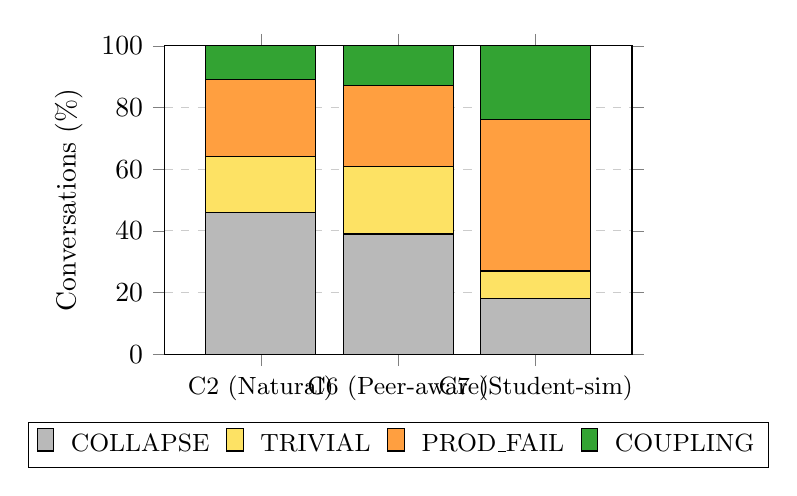
\begin{tikzpicture}
  \begin{axis}[
    ybar stacked,
    bar width=1.4cm,
    width=0.62\textwidth,
    height=5.5cm,
    ymin=0, ymax=100,
    ylabel={Conversations (\%)},
    xtick={1,2,3},
    xticklabels={C2 (Natural), C6 (Peer-aware), C7 (Student-sim)},
    xticklabel style={font=\small},
    legend style={at={(0.5,-0.22)}, anchor=north, legend columns=4,
                  font=\small, column sep=4pt},
    enlarge x limits=0.35,
    ymajorgrids=true,
    grid style={dashed, gray!40},
    tick align=outside,
    every axis plot/.append style={draw=black, line width=0.4pt},
  ]
  % COLLAPSE (bottom, gray) — C2:46, C6:39, C7:18
  \addplot[fill=gray!55] coordinates {(1,46) (2,39) (3,18)};
  % TRIVIAL (yellow) — C2:18, C6:22, C7:9
  \addplot[fill=yellow!70!orange!60] coordinates {(1,18) (2,22) (3,9)};
  % PROD_FAIL (orange) — C2:25, C6:26, C7:49
  \addplot[fill=orange!75] coordinates {(1,25) (2,26) (3,49)};
  % COUPLING (green, top) — C2:11, C6:13, C7:24
  \addplot[fill=green!55!black!80] coordinates {(1,11) (2,13) (3,24)};
  \legend{COLLAPSE, TRIVIAL, PROD\_FAIL, COUPLING}
  \end{axis}
  \end{tikzpicture}
  \caption{Quadrant distribution across conditions. Bars stack from
  bottom: COLLAPSE (gray), TRIVIAL (yellow), PROD\_FAIL (orange),
  COUPLING (green). The dominant shift from C2/C6 to C7 is a transfer
  of mass from COLLAPSE to PROD\_FAIL and COUPLING, driven by the
  Phase~A activation effect (Section~\ref{sec:results}).}
  \label{fig:quadrants}
\end{figure}

\subsection{Epistemic Decomposition: Agent Epistemic Contribution}
\label{sec:aec}

The metrics presented so far measure \emph{how much} agents collaborate
(\CDI) and \emph{how deeply} they engage across phases (\CQI, \PhAQ).
They do not answer a more fundamental question: was collaboration
epistemically \emph{necessary}---that is, did the pair achieve a result
neither agent could reach alone? We address this via a Shapley-value
decomposition we term \textbf{Agent Epistemic Contribution (\AEC)}.

\paragraph{Setup.}
For each of the $140$ benchmark problems we run each agent in isolation
with only its own \CIDI{} packet, using the same model (GPT-4.1) and
temperature ($T = 0$) as the collaborative sessions, and the same
maximum token budget per turn. Three value functions are defined (each
$\in \{0, 0.5, 1\}$ following a partial-credit scale):
\[
  v(\{A\}),\quad v(\{B\}),\quad v(\{A,B\}) = \text{best C7 replication correctness}.
\]
We use the best C7 replication as $v(\{A,B\})$ to obtain an upper
bound on what the pair can achieve under the strongest framing; this
means the resulting \EN{} and \CS{} estimates should be interpreted
as \emph{upper-bound measures of activated interdependence under C7},
not as estimates applicable to C2 or C6. Shapley values for $N=2$ are:
\[
  \AEC_A = \tfrac{1}{2}v(\{A\}) + \tfrac{1}{2}(v(\{A,B\}) - v(\{B\})),\quad
  \AEC_B = \tfrac{1}{2}v(\{B\}) + \tfrac{1}{2}(v(\{A,B\}) - v(\{A\})).
\]
We derive three aggregate measures. \textbf{\EN{} (Epistemic
Necessity)}: $v(\{A,B\}) > \max(v(\{A\}), v(\{B\}))$, i.e., the C7
pair surpasses the better solo. \textbf{\CS{} (Collaborative Surplus)}:
$v(\{A,B\}) - \max(v(\{A\}), v(\{B\}))$, the magnitude of the gain.
\textbf{EB (Epistemic Balance)}: $1 - |\AEC_A - \AEC_B|$, symmetry of
contribution. The \AEC{} decomposition separates two distinct notions
of interdependence: \emph{structural} interdependence, encoded in the
task design (both-solo-zero $= 85\%$), and \emph{activated}
interdependence under the optimal framing (EN rate $= 25\%$ under C7).
This distinction is not visible in \CDI{} alone and has direct
implications for benchmark diagnosis.

\paragraph{Results.}
Table~\ref{tab:aec} summarises the decomposition. Solo correctness is
very low: $v_A = 0.100$, $v_B = 0.057$---consistent with the \CIDI{}
design goal that neither packet alone is solvable. The C7 pair achieves
$v_{AB} = 0.357$, a $3.6\times$ improvement over the better individual.
Critically, $85\%$ of problems exhibit \emph{both-solo-zero}: neither
packet provides sufficient information for any correct answer, validating
the \CIDI{} epistemic filter at the correctness level. \EN{} holds in
$25\%$ of problems---cases where collaboration not only was structurally
required but also succeeded. Mean \CS{} $= +0.207$ and mean EB $=
0.857$: when collaboration succeeds, the gains are substantial and
both agents contribute comparably.

\begin{table}[t]
  \caption{\AEC{} decomposition across $140$ problems. \emph{Both-solo-zero}:
  neither agent's packet alone permits a correct answer; \EN: pair
  surpasses the better solo; \CS: collaborative surplus over best solo;
  EB: Shapley balance between agents.}
  \label{tab:aec}
  \centering
  \begin{tabular}{lr}
    \toprule
    \textbf{Metric} & \textbf{Value} \\
    \midrule
    $v_A$: Agent A solo correctness  & 0.100 \\
    $v_B$: Agent B solo correctness  & 0.057 \\
    $v_{AB}$: C7 pair correctness    & 0.357 \\
    \midrule
    Both-solo-zero rate              & 85.0\% \\
    \EN{} rate (epistemic necessity) & 25.0\% \\
    \CS{} mean (collaborative surplus)  & $+0.207$ \\
    EB mean (epistemic balance)      & 0.857  \\
    \bottomrule
  \end{tabular}
\end{table}

\paragraph{Connecting AEC to framing.}
The \AEC{} decomposition surfaces a structural gap that \CDI{} alone
cannot reveal. All 140 problems have structural interdependence encoded
by the \CIDI{} design ($85\%$ both-solo-zero): neither agent's packet
suffices for a correct answer, so collaboration is a mathematical
necessity. Yet even under the \emph{strongest} framing (C7), only
$25\%$ of these structurally interdependent problems achieve epistemic
necessity---the pair surpasses the better solo. The gap between $85\%$
structural and $25\%$ activated is not a claim about C2 behavior (we
did not run AEC under C2); it is a claim about how much latent
collaborative capacity remains unexploited even under optimal framing.
The interpretation is that the \CIDI{} split reliably creates the
\emph{conditions} for collaboration, but converting those conditions
into activated epistemic necessity requires both the right framing and
sufficient problem-solving capacity. For benchmark designers, this
structural/activated gap quantifies how much additional value a better
framing or coordination mechanism could unlock on this class of
problems: the ceiling is $85\%$ (all both-solo-zero problems becoming
activated), and the current optimum is $25\%$.

\subsection{Hypothesis 3: Descriptive Robustness Across Subject and Difficulty}

To assess descriptive robustness, we computed mean \CDI{} for each of
the 30 subject $\times$ difficulty cells (Appendix~\ref{app:heatmap}).
C7 numerically outperforms C2 in all 30 cells, but per-cell $n$ values
are small (range 1--8, mean 4.7), and cells with $n < 3$ do not permit
reliable effect-size estimation. \textbf{This constitutes descriptive
robustness, not formal cell-level generalization}: no per-cell test
survives multiplicity correction, and the H3 claim should be read as
``the aggregate advantage is consistent in direction across the
taxonomy'' rather than ``the effect is demonstrated in each cell
independently.'' Effect sizes in cells with $n \geq 3$ range from
$d = 0.63$ (Counting \& Probability, Level~2) to $d = 2.51$ (Algebra,
Level~2), with larger effects at higher difficulty levels---directionally
consistent with framing mattering most when the problem genuinely
requires coordinated reasoning (full table in Appendix~\ref{app:heatmap}).

The C6 vs.\ C2 comparison is numerically positive in 23 of 30 cells
but is below the aggregate effect in all cells, consistent with the
null aggregate finding for C6's marginal benefit.

\subsection{Robustness and Validity Checks}

\paragraph{W2 — C6 rules out partner-awareness, not ignorance.}
A potential concern is that C7 confounds active-learner role framing
with simulated ignorance: the student-role prompt instructs agents both
to adopt a collaborative-learner stance \emph{and} to acknowledge that
they do not know the answer. The C6 condition partially addresses this.
C6 establishes explicit partner-awareness without any learner-role
component; if simulated ignorance alone explained C7's gains, C6
should also outperform C2, since C6 agents equally lack access to the
full solution. The negligible C6 vs.\ C2 effect ($d=0.16$,
$\Delta_{\CDI} = +0.028$, $p = 0.026$, not surviving Bonferroni
correction) rules out partner-awareness as the mechanism. However, C6
does \emph{not} fully isolate the active-learner communicative-stance
component from the instruction to withhold expert-like certainty: a framing that says
``reason cautiously, you may not have the full answer'' (without the
collaborative learner persona) could also fail to improve over C2 for
different reasons. The precise subcomponent responsible requires an
ignorance-only ablation (e.g., ``you do not know the answer; reason
carefully'' without active-learner collaboration directives), which is
identified as a key next experiment in Section~\ref{sec:future_ablations}.

\paragraph{W3 — CDI and correctness are orthogonal (by design).}
A reviewer might ask whether \CDI{} predicts solution correctness.
Across all 1,967 conversations, $P(\text{correct} \mid \CDI \geq 0.5)
= 0.321$ vs.\ $P(\text{correct} \mid \CDI < 0.5) = 0.324$---a
difference of $-0.003$ ($\chi^2 = 0.01$, $p = 0.94$). This
orthogonality is \emph{theoretically expected}: \CDI{} measures
process quality, not solution quality. Productive failure theory
\citep{kapur2016examining} explicitly predicts that deep collaborative
engagement does not guarantee correct outcomes, particularly on
problems selected for their difficulty. The appropriate metric for
practical impact is the \textsc{Coupling} rate, where both deep
process and correct outcome co-occur. C7 achieves a Coupling rate of
$24\%$ vs.\ $11\%$ (C2) and $13\%$ (C6)---a $2.2\times$ improvement
over the baseline achieved with the \emph{same mean conversation length}
(C2: 19.9 turns, C6: 20.0, C7: 19.9). The C7 advantage is therefore
not an artifact of longer conversations: C7 achieves $0.031$ \CDI{}
per turn, $69\%$ more than C2 ($0.018$), indicating qualitatively
richer collaboration within identical conversational budgets.

\paragraph{W4 — Convergent validity with DAG-weighted \CDI.}
The uniform $1/12$ weighting of \CDI{} treats all 12 cells equally,
but PISA process depth (A $\to$ B $\to$ C $\to$ D) and competency
sophistication (1 $\to$ 2 $\to$ 3) define a natural topological order.
We computed a DAG-weighted variant $\CDI_w = \sum_{i} w_i \cdot
\mathbb{1}[c_i = 1]$ where $w_i \propto \text{phase\_depth}(i) \times
\text{comp\_depth}(i)$, normalized to sum to one (range: $w_{A1} =
0.017$ to $w_{D3} = 0.200$). The condition rankings are identical:
$\CDI_w$ = 0.369, 0.397, 0.601 for C2, C6, C7---compared to uniform
\CDI{} = 0.362, 0.390, 0.613. The near-perfect rank-order agreement
(Spearman $\rho > 0.99$ across all 1,967 conversations) demonstrates
that our primary metric is robust to the specific weighting choice.
Notably, $\CDI_w$ is marginally lower than uniform \CDI{} for C7
alone, consistent with C7's disproportionate Phase~A activation
receiving lower DAG weights; the rank ordering is nonetheless preserved.

\paragraph{W5 — Statistical power and confidence intervals.}
Bootstrap resampling ($B = 10{,}000$) of the per-problem mean
$\CDI(\text{C7}) - \CDI(\text{C2})$ difference yields a $95\%$
confidence interval of $[0.219, 0.284]$---entirely above zero and
bounded away from the C6 effect ($\Delta = 0.028$). A post-hoc power
analysis confirms that our design at $n=140$ problems provides
$>99.9\%$ power to detect the observed effect size ($d = 1.30$) at
$\alpha = 0.05$; formally, $n = 5$ problems would suffice for $80\%$
power at this effect size. Within-problem replication variance
($\sigma_{\text{within}} \approx 0.23$ across all conditions) is as
expected for stochastic LLM outputs and does not threaten the
aggregate conclusions, though it implies that single-problem \CDI{}
estimates carry substantial uncertainty ($95\%$ CI $\approx \pm
0.26$).

% ================================================================
\subsection{Ablation Conditions: C\textsubscript{FULL} and C\textsubscript{EXP}}
\label{sec:ablations}

To disentangle the active-learner communicative stance from the \CIDI{}
structural split, we ran two ablation conditions on the full 140-problem
corpus (3 replications each, 840 conversations total):
\textbf{C\textsubscript{FULL}} applies C7 active-learner framing with
full problem context (both agents see the complete problem; no information
split), and \textbf{C\textsubscript{EXP}} applies the \CIDI{} split with
expert-solver framing instead of the active-learner stance.

Table~\ref{tab:ablations} shows mean \CDI{} and quadrant rates across
all five conditions.

\begin{table}[ht]
  \caption{Mean \CDI{} and quadrant distribution across main and ablation
  conditions ($n = 140$ problems). Both ablation conditions fall \emph{below}
  C2, the natural-framing baseline, indicating that neither component alone
  accounts for the C7 effect.}
  \label{tab:ablations}
  \centering
  \begin{tabular}{lrrrrr}
    \toprule
    \textbf{Condition} & \textbf{Mean \CDI{}} & \textbf{COUPLING} & \textbf{PROD\_FAIL} & \textbf{TRIVIAL} & \textbf{COLLAPSE} \\
    \midrule
    C7 (CIDI + learner)       & $0.613 \pm 0.014$ & 24\% & 49\% &  9\% & 18\% \\
    C6 (CIDI + peer-aware)    & $0.390 \pm 0.015$ & 13\% & 26\% & 22\% & 39\% \\
    C2 (CIDI + natural)       & $0.362 \pm 0.015$ & 11\% & 25\% & 18\% & 46\% \\
    \midrule
    C\textsubscript{FULL} (learner, no split) & $0.296 \pm 0.018$ & 11\% & 12\% & 49\% & 28\% \\
    C\textsubscript{EXP} (expert + split)     & $0.267 \pm 0.017$ &  5\% & 17\% & 25\% & 53\% \\
    \bottomrule
  \end{tabular}
\end{table}

Both ablation conditions fall \emph{below} C2 (the natural-framing
baseline with \CIDI{} split): C\textsubscript{FULL} achieves mean
$\CDI = 0.296 \pm 0.018$ ($d = -0.33$ vs.\ C2) and C\textsubscript{EXP}
achieves $0.267 \pm 0.017$ ($d = -0.49$ vs.\ C2). Neither approaches
C7 (C\textsubscript{FULL}: $d = 1.63$; C\textsubscript{EXP}: $d = 1.87$).
Three findings emerge from the quadrant profiles.

\textbf{(1) The \CIDI{} split is necessary, not redundant.} Removing
the information split while retaining C7 framing (C\textsubscript{FULL})
raises the TRIVIAL rate to $49\%$: both agents independently solve the
problem without epistemically needing each other's contribution. The
active-learner register alone cannot manufacture the structural need
to share information; that need must arise from the task design.

\textbf{(2) The active-learner stance is specifically required, not just
any strong framing.} Replacing C7 with expert-solver framing
(C\textsubscript{EXP}) while retaining the \CIDI{} split produces $53\%$
COLLAPSE---the highest collapse rate across all five conditions. The
expert-solver role suppresses the epistemic inquiry behaviors (Phase A
activation, explicit uncertainty, question-asking) that \CDI{} captures,
even when the structural information asymmetry is in place.

\textbf{(3) The two components are synergistic.}
C\textsubscript{FULL} and C\textsubscript{EXP} are not meaningfully
different from each other ($d = 0.14$), confirming that neither component
alone explains the C7 effect. It is their combination---structural
interdependence \emph{and} an active-learner communicative stance---that
produces the shift from COLLAPSE to COUPLING and PROD\_FAIL observed
under C7. This rules out two simpler explanations: that any learner-like
register suffices without genuine information need, and that any strong
role instruction activates collaborative depth when epistemic structure
is present.

% ================================================================
\section{Discussion}
\label{sec:discussion}

\paragraph{The C6 $\approx$ C2 finding: partner-awareness is not sufficient.}
The near-equivalence of C2 and C6 carries a clear design implication
within this regime. Several multi-agent systems rely on agents being
\emph{told} that they are collaborating with a peer
\citep{liang2023encouraging, du2023improving}; our results indicate
that this manipulation leaves the agent's default behavioral
mode---expert-answering---largely intact in the \CIDI-amenable regime.
What appears to counteract this default, in the present setting, is an
active-learner communicative stance that makes producing an authoritative
answer explicitly inappropriate, shifting agents toward questioning,
uncertainty expression, and joint model-building. For benchmark
designers, this suggests that collaborative-framing ablations should
manipulate epistemic communicative stance, not merely task awareness,
to produce measurable \CPP{} differences---though future ablations
(Section~\ref{sec:future_ablations}) are needed to confirm that this
effect is specific to the active-learner component rather than any
strong role instruction.

\paragraph{Structural vs.\ activated interdependence: implications for benchmark design.}
The structural/activated distinction surfaced by \AEC{} has direct
consequences for how multi-agent benchmarks should be designed and
interpreted. A benchmark can guarantee structural interdependence
($85\%$ both-solo-zero in our corpus) while still leaving a large
fraction of that structure unactivated even under the strongest framing
($25\%$ EN under C7). This $60$-percentage-point gap is invisible to
accuracy-based metrics but fully captured by \AEC{}. For practitioners
designing information-split benchmarks, \AEC{} thus provides an
interpretable audit: high both-solo-zero with low \EN{} signals that
agents are failing to exploit the task's collaborative structure, and
the gap quantifies how much additional value a better framing or
coordination mechanism could theoretically unlock.

\paragraph{Ablation results: structural interdependence and active-learner stance are jointly necessary.}
\label{sec:future_ablations}
The two ablation conditions (Section~\ref{sec:ablations}) resolve the
main mechanistic ambiguity in the three-condition design.
C\textsubscript{FULL} (learner framing, no \CIDI{} split) achieves
$\CDI = 0.296$, falling below the natural-framing baseline C2
($\CDI = 0.362$), with $49\%$ of conversations classified as TRIVIAL:
agents possessing the same information solve in parallel rather than
collaborating. This confirms that structural information asymmetry is
a necessary condition, not an implementation detail. C\textsubscript{EXP}
(expert-solver framing with \CIDI{} split) achieves $\CDI = 0.267$, the
lowest of all five conditions, with $53\%$ COLLAPSE: expert framing
suppresses the inquiry behavior that \CDI{} captures even when the
epistemic structure is in place. Together, these results confirm that
C7's effect ($\CDI = 0.613$, $d = 1.45$ vs.\ C2) arises from a
synergistic combination of structural interdependence and active-learner
communicative stance, not from either component individually.

Two ablations remain as future work: a \textbf{debate/critique condition}
(C\textsubscript{DEB}: CIDI split with adversarial framing) to test
whether productive disagreement structures also activate \CDI; and an
\textbf{ignorance-only condition} (``reason cautiously; you may not have
all the information,'' without collaboration directives) to isolate the
uncertainty-acknowledgement subcomponent from the full C7 instruction.
Per-condition \AEC{} runs would additionally allow direct comparison of
activated epistemic necessity across C2, C6, and C7.

\paragraph{Productive failure and benchmark interpretation.}
The large PROD\_FAIL mass under C7 ($49\%$) invites careful
interpretation and is not a failure of the framing. PROD\_FAIL
conversations exhibit high collaborative depth ($\CDI \geq 0.5$) but
reach an incorrect conclusion---they represent \emph{genuine}
collaborative engagement with hard problems that exceed current
reasoning capacity. This is a direct consequence of the corpus design:
Phase~1 selected for problems that challenge even deep collaboration,
so a high PROD\_FAIL rate is the expected outcome of a well-functioning
collaborative framing on a hard benchmark. The evaluatively important
comparison is against COLLAPSE ($46\% \to 18\%$ from C2 to C7): that
transition represents conversations that added neither process nor
outcome value. The COUPLING rate ($11\% \to 24\%$) measures the
achievable ceiling under the current model and corpus. For benchmark
designers, this three-quadrant shift (COLLAPSE $\to$ PROD\_FAIL
$\to$ COUPLING) provides a richer picture of framing effectiveness
than accuracy alone: it distinguishes \emph{productive engagement with
hard problems} from \emph{collapse due to insufficient framing}.
In human learning contexts, productive failure is associated with
superior transfer \citep{kapur2016examining, schwartz1998time};
whether LLM-generated PROD\_FAIL trajectories carry analogous value
in human-AI hybrid settings is an open empirical question.

\paragraph{Limitations.}
Several limitations bound the current conclusions.
\emph{(L1) Corpus conditionality}: the 140-problem corpus was filtered
using C7 performance, so all estimates are conditional on
\CIDI-amenable problems. Because the corpus favours problems where C7
succeeds, the observed effect sizes may overestimate the framing
benefit expected on an unfiltered MATH sample. This is the most
important methodological caveat; all conditional claims are presented
accordingly in Section~\ref{sec:design}.
\emph{(L2) Remaining ablation scope}: the C\textsubscript{FULL} and
C\textsubscript{EXP} ablations (Section~\ref{sec:ablations}) confirm
that the C7 effect requires the joint presence of structural
interdependence and active-learner framing. The remaining gap concerns
\emph{subcomponents} of the C7 instruction: an ignorance-only condition
(``reason cautiously without claiming certainty,'' without collaboration
directives) would isolate the uncertainty-acknowledgement component from
the collaborative-inquiry component, and a debate condition would test
adversarial framing as an alternative activation mechanism.
\emph{(L3) AEC scope}: $v(\{A,B\})$ uses the best C7 replication; EN
and CS are therefore upper-bound estimates under the strongest framing
and cannot be directly compared across conditions without per-condition
AEC runs.
\emph{(L4) Model generalisability}: all agents use GPT-4.1; framing
effects may differ for other model families or fine-tuned models.
\emph{(L5) Reliability sample}: the reliability evidence is
preliminary ($n=36$); per-cell $\kappa$ estimates require $\geq 100$
conversations.
\emph{(L6) Collaborative register vs.\ reasoning}: we cannot rule out
that C7 agents produce high-\CDI{} discourse without the underlying
reasoning structure that \CPP{} assumes; micro-level trace analysis is
needed.

% ================================================================
\section{Conclusion}
\label{sec:conclusion}

We introduced the \CPP{} evaluation framework and the \CIDI{}
benchmark to measure how deeply LLM agents collaborate, and used them
to show that epistemic role framing---instructing agents to adopt an
active-learner stance---shifts behaviour decisively from
expert-answering to collaborative sense-making ($d = 1.30$ on \CDI;
COUPLING rate more than doubles). Partner-awareness alone does not
produce this shift ($d = 0.16$, not significant after Bonferroni
correction), and the effect is numerically positive across all 30
subject-difficulty cells of the benchmark (descriptive; per-cell samples
are small). The \AEC{} Shapley decomposition further reveals that the
\CIDI{} split reliably creates structural interdependence ($85\%$
both-solo-zero), and that even under the strongest framing only $25\%$
of that structure becomes activated epistemic necessity---a gap that
accuracy-based evaluation cannot surface.

These results carry two principal implications for the \textbf{E\&D}
community. For evaluation, they demonstrate that \CDI{} and the
structural/activated interdependence distinction are useful additions
to accuracy when benchmarking collaborative agents: accuracy conflates
COUPLING with TRIVIAL and misses PROD\_FAIL entirely. For design, they
show that active-learner communicative-role framing is an effective
intervention in the CIDI-amenable regime, producing substantially
stronger collaborative discourse than partner-awareness alone; whether
this advantage generalises beyond the selected corpus requires further
validation.

Two ablation conditions (C\textsubscript{FULL}: learner framing without
\CIDI{} split; C\textsubscript{EXP}: expert framing with \CIDI{} split)
confirm that the C7 effect is synergistic: neither structural
interdependence nor active-learner stance alone accounts for the
observed \CDI{} gain, and expert framing with the split produces the
\emph{highest} collapse rate across all conditions ($53\%$ COLLAPSE).
Three extensions will most sharpen this work: (1) subcomponent ablations
(ignorance-only condition, debate framing) to isolate specific elements
of the C7 instruction; (2) per-condition \AEC{} runs to directly measure
how activated epistemic necessity varies across C2, C6, and C7; and (3)
developing automated \CPP{} scoring via LLM judges to enable reliability
sample expansion and annotation at scale. An anonymized review release covering the
full artifact suite is available (see Artifact Availability section).

% ================================================================
\section*{Artifact Availability}
\label{sec:artifacts}

To support reproducibility and to fulfil E\&D benchmark contribution
requirements, we provide an anonymized review release at
\url{[anonymous repository — redacted for review]} containing:

\begin{itemize}
  \item \textbf{CPP rubric}: complete 12-cell annotation rubric with
  anchor descriptors, boundary cases, and annotator guidelines for all
  cells.
  \item \textbf{CIDI generation prompt}: the full structured prompt
  template and validation logic used to generate and quality-filter
  information splits.
  \item \textbf{Problem corpus}: the 140 \CIDI{} split triples (Shared
  context / Packet A / Packet B), identified by MATH benchmark ID.
  Original problem text is not redistributed in compliance with the
  MATH benchmark license; MATH IDs and our derived splits are
  provided.
  \item \textbf{Conversation transcripts}: full turn-by-turn logs for
  all 1,967 conversations across C2, C6, and C7 conditions.
  \item \textbf{CPP annotations}: annotator scores for all 12 cells,
  raw disagreement records, and consensus resolutions for the 36
  reliability conversations.
  \item \textbf{Scoring scripts}: CPP metric computation (CDI, CQI,
  PhAQ, ATC, CY) and quadrant assignment.
  \item \textbf{AEC scripts}: solo-run correctness evaluation and
  Shapley-value computation.
  \item \textbf{Benchmark card}: documentation of corpus construction,
  selection conditionality, intended use, known limitations, and
  metadata.
\end{itemize}

The final public release will be hosted with persistent identifiers.
All annotations, scripts, and derived data are released under CC BY
4.0; conversation logs under the terms of the applicable API provider.

% ================================================================
\section*{Acknowledgements}
This work was supported in part by [Funding agency redacted for
anonymous review]. We thank the research assistants who provided
annotation for the \CPP{} rubric. Compute was provided by [HPC
resource redacted for anonymous review].

\bibliography{references}

% ================================================================
\appendix

\section{CPP Annotation Rubric}
\label{app:rubric}

Each of the 12 cells $(P, C)$ for $P \in \{A, B, C, D\}$ and
$C \in \{1, 2, 3\}$ is scored on a 0--3 scale. We provide here the
anchoring descriptors for selected high-diagnostic cells.

\paragraph{Cell A1 (Exploring \& Understanding / Shared Understanding).}
\textbf{0}: No evidence that agents jointly discussed the problem;
one agent simply began solving. \textbf{1}: Agents acknowledged the
problem exists and restated it, but no reconciliation of perspectives.
\textbf{2}: Agents explicitly compared what each knows and flagged
gaps; at least one question about the other's packet was asked and
answered. \textbf{3}: Full joint problem model constructed; both
agents articulate a shared interpretation that differs from what
either could have produced alone, and this model visibly shapes the
subsequent solution strategy.

\paragraph{Cell D3 (Monitoring \& Reflecting / Team Organisation).}
\textbf{0}: No meta-discussion of the collaborative process or
strategy; agents proceed to output without review. \textbf{1}: One
agent flags a potential error but the flag is ignored by the partner.
\textbf{2}: Agents engage in a substantive exchange about whether
their approach is working; at least one revision of strategy is
proposed. \textbf{3}: Agents explicitly evaluate the quality of their
collaboration itself (e.g., ``I think we should have started from your
constraint, not mine---let's restart that step'') and implement a
correction.

\paragraph{Full rubric.} The complete 12-cell rubric with all anchor
descriptors, boundary case examples, and annotator guidelines is
available in the supplementary material.

\section{CIDI Generation Prompt}
\label{app:cidi_prompt}

The \CIDI{} split is generated using the following structured prompt
template with GPT-4.1 at temperature 0. The prompt instructs the
generator to:
\begin{enumerate}
  \item Identify the core mathematical objects and relations in the
  problem.
  \item Partition those objects into two groups such that group~A
  provides the structural constraints and group~B provides the
  quantitative anchors (or a domain-appropriate analogue).
  \item Verify that a solver with only group~A information cannot
  determine the numerical answer even with unlimited mathematical
  knowledge, and vice versa.
  \item Express each packet in natural language, avoiding explicit
  statements of what is absent from the other packet.
\end{enumerate}
The generated split is validated by running a single GPT-4.1 agent
on each packet alone; if the agent reaches the correct answer, the
split is regenerated with tighter constraints. Typical regeneration
rate was $12\%$ of problems.

\section{Pilot Study: Condition Selection}
\label{app:pilot}

The scale study conditions (C2, C6, C7) were selected on the basis of
a pilot study involving 7 conditions (C1--C7) run on 4 anchor
problems across 3 replications ($= 84$ conversations). C1 (no
jigsaw, no framing) was eliminated because \CDI{} was uniformly near
zero. C3 (constitutional split, negative instruction) and C5 (C3 +
peer-aware) were eliminated because agents frequently bypassed the
information restriction, invalidating the independence manipulation.
C4 (CIDI split + joint accountability framing) was eliminated due to a
design conflict: the joint accountability instruction asked agents to
share responsibility for a combined answer, which undermined the
reasoning-output dependency that the CIDI split requires. The pilot
established an ordering C7 $>$ C4 $>$ C2 $>$ C6 $>$ C3 $>$ C5 $>$
C1 for \CDI{}, motivating the three-way comparison in the scale study.
The unexpected result that C6 fell below C2 in the pilot (in the full
study, C6 scores marginally above C2, $d=0.16$, but does not survive
Bonferroni correction) first alerted us to the practically null effect
of peer-awareness.

\section{Subject-Level Generalisability Results}
\label{app:heatmap}

Table~\ref{tab:heatmap} reports mean \CDI{} for each of the 30
subject $\times$ difficulty cells under conditions C2 and C7. C7
numerically outperforms C2 in all 30 cells. Cell $n$ values range from
1 to 8 (mean 4.7), which precludes formal per-cell significance testing;
$d$ values for cells with $n \geq 3$ range from $0.63$ to $2.51$.
Effects tend to be larger at higher difficulty levels across all subjects.

\begin{table}[h]
  \caption{Cell-level \CDI{} means and Cohen's $d$ (C7 vs.\ C2) for
  all 30 subject $\times$ difficulty combinations. $d$ is omitted for
  $n < 3$ (insufficient data). Subject labels follow MATH benchmark
  categories \citep{hendrycks2021math}.}
  \label{tab:heatmap}
  \centering
  \small
  \begin{tabular}{llrrrr}
    \toprule
    \textbf{Subject} & \textbf{Level} & \textbf{$n$} &
    \textbf{CDI (C2)} & \textbf{CDI (C7)} & \textbf{$d$} \\
    \midrule
    Algebra         & 1 &  4 & 0.342 & 0.667 & 2.09 \\
    Algebra         & 2 &  3 & 0.333 & 0.711 & 2.51 \\
    Algebra         & 3 &  2 & 0.333 & 0.517 & --- \\
    Algebra         & 4 &  7 & 0.386 & 0.557 & 1.38 \\
    Algebra         & 5 &  6 & 0.378 & 0.647 & 2.06 \\
    \midrule
    Geometry        & 1 &  5 & 0.360 & 0.483 & 1.25 \\
    Geometry        & 2 &  4 & 0.325 & 0.568 & 1.60 \\
    Geometry        & 3 &  6 & 0.305 & 0.536 & 1.19 \\
    Geometry        & 4 &  6 & 0.268 & 0.644 & 1.53 \\
    Geometry        & 5 &  6 & 0.306 & 0.619 & 2.29 \\
    \midrule
    Number Theory   & 1 &  1 & 0.367 & 0.833 & --- \\
    Number Theory   & 2 &  5 & 0.326 & 0.546 & 0.73 \\
    Number Theory   & 3 &  6 & 0.290 & 0.496 & 2.77 \\
    Number Theory   & 4 &  5 & 0.364 & 0.659 & 0.90 \\
    Number Theory   & 5 &  8 & 0.409 & 0.669 & 0.91 \\
    \midrule
    Prealgebra      & 1 &  3 & 0.306 & 0.428 & 1.81 \\
    Prealgebra      & 2 &  6 & 0.403 & 0.581 & 1.14 \\
    Prealgebra      & 3 &  7 & 0.399 & 0.676 & 2.18 \\
    Prealgebra      & 4 &  4 & 0.336 & 0.558 & 1.30 \\
    Prealgebra      & 5 &  4 & 0.383 & 0.606 & 0.91 \\
    \midrule
    Precalculus     & 1 &  2 & 0.462 & 0.517 & --- \\
    Precalculus     & 2 &  3 & 0.342 & 0.606 & 1.86 \\
    Precalculus     & 3 &  6 & 0.325 & 0.508 & 0.78 \\
    Precalculus     & 4 &  7 & 0.431 & 0.717 & 1.73 \\
    Precalculus     & 5 &  5 & 0.424 & 0.737 & 1.14 \\
    \midrule
    Probability     & 1 &  1 & 0.567 & 0.817 & --- \\
    Probability     & 2 &  4 & 0.439 & 0.587 & 0.63 \\
    Probability     & 3 &  2 & 0.556 & 0.867 & --- \\
    Probability     & 4 &  5 & 0.271 & 0.609 & 1.30 \\
    Probability     & 5 &  7 & 0.375 & 0.685 & 1.38 \\
    \bottomrule
  \end{tabular}
\end{table}

\end{document}
